\chapter{Dataset}
Some teams participating in GIVE Challenge tried to learn either language expression or decision-making process from a human-human interactions in GIVE scenario. They were however relying on a small self-collected datasets. In a light of this, organizers of GIVE Challenge decided they would collect and provide dataset for future use. This chapter serves as an introduction and analysis of this dataset.

As a side note, \citet{striegnitz2012referring} report on a smaller German dataset, which is similar to the one I will be talking about. 

In the first section, I will introduce the dataset and provide technical details of how it was created. Second section, will, after the fashion of GIVE Challenge look how world and demographic factors influenced the task performance.

\section{General overview}
The data-collection started in July and finished November of 2012. Through that period 21 interactions between two human subjects were recorded. Originally, 22 pairs participated, but one of the pair failed to finish the tasks and is excluded from the dataset. The subjects were asked to bring someone they know and they were financially compensated for the effort. 

The set-up for the experiment is in the figure \ref{fig:give-experiment-setup}. One human subject was an instruction giver (IG). He is on the right in the figure \ref{fig:give-experiment-setup}. His role was essentially the role of NLG system in GIVE Challenge. He was able to see a map of the world, which was updated real-time and informed of all necessary steps to finish the task. In addition, he was able to see the other's person client screen. He communicated with the other person through a microphone and his goal
was to navigate the other person through the world and make him finish the treasure-hunt.

\begin{figure}[h]
  \centering
	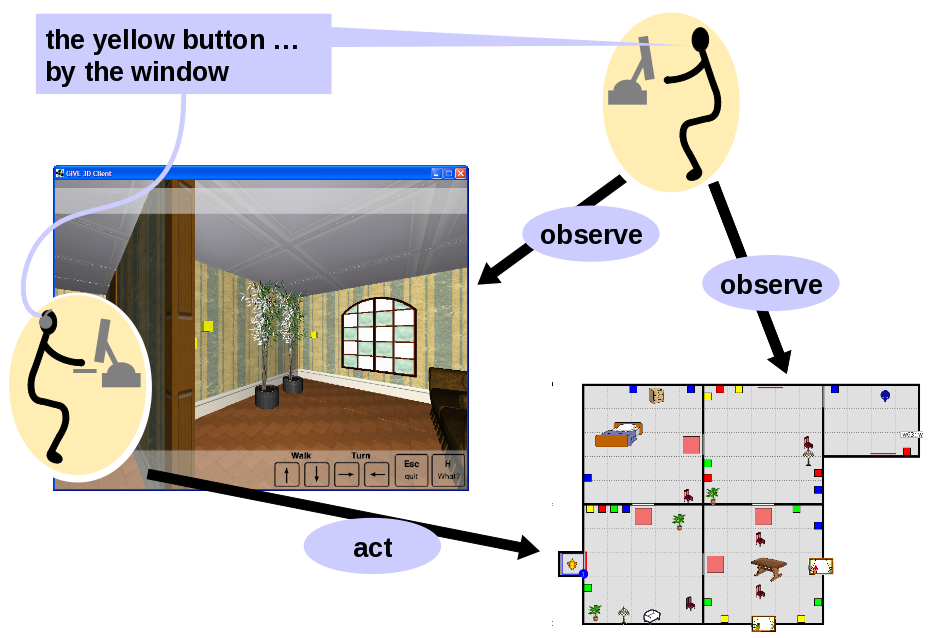
\includegraphics[width=0.7\textwidth]{Images/experiment-set-up}
	\caption{Experiment set-up of data collection}
	\label{fig:give-experiment-setup}
\end{figure}

The other person was an instruction follower (IF). He is on the left in the figure \ref{fig:give-experiment-setup}. He interacted with the client and listened to IG's instructions through a headset.

Each pair did one short tutorial world and after that, they switched roles of instruction giver and instruction follower. Following was one world randomly chosen from two variants (marked with 1 or 3). Finally they did a difficult version of the  second variant (1-d or 3-d). A difficult version of the world had an increased number of distracting buttons and landmarks compared to the ``normal'' version. If not present in the report or not stated otherwise, the short tutorial worlds are normally excluded from the statistics.

Similarly to the GIVE Challenge, after all 3 rounds subjects were asked to fill a questionnaire. Its purpose was to get demographic information on subjects. Age, gender,  gaming experience, previous cooperation between IG and IF and ability to navigate in the world were part of the questionnaire. To measure the ability to navigate in the world the Santa Barbara Sense of Direction (SBSOD) scores were used \citet{hegarty2002development}.

As was mentioned in chapter \ref{chap:give-challenge}, the entire session is logged to the database. The player's position, orientation and all visible objects are logged at fixed rate. Moreover, other information as buttons presses or an end of a session are also stored in the logs. Because the worlds are static, distances and angles between player and other game's objects are easily computed from there.

Apart from logs, there are of course sound files of IG giving directions. These were transcribed and together with the logs transformed into an ELAN files. ELAN is an annotation software \citep{sloetjes2008annotation}. I will use a term automatic annotations for these files. 

Building on top of these automatic annotations are manual annotations. They are primarily concerned with referring expressions and also stored in ELAN format. Most referring expressions in GIVE aim to locate a button, which needs to be pressed. I will call the button, which is a goal of an referring expression, the target button. Which button is the target button of a reference is among the manual annotations. Next layer of the annotations is some basic grouping of the references. Whether it is a reference to a single button, group of button, to a landmark and so on. Third layer looks deeper into the contents of the reference. It notes whether the reference contains for example the color of a button, whether distractors or landmarks are part of the reference or whether the reference points out that a button was already pressed before.

Previously mentioned logs, automatic annotations and manual annotations together form the dataset this chapter is dealing with.

An example of what can be extracted from the data is in the following text. Spatial information are transcribed in parentheses for a sake of clearness.

\begin{verse}
(IF enters a room)\\
IG: Go towards the red buttons.\\
(IF turns right and start walking, but he turns too much)\\
IG: No the ones next to the lamp...\\
(IF corrects his direction)\\
IG: Yeah that lamp. On the right.\\
(IF is facing three buttons.)\\
IG: Press the button on the wall you are looking at, that's far from the lamp and on the left. \\
(IF goes towards the correct button and stops close to him)\\
IG: Press it.\\
\end{verse}

\section{World and Demographic factors}
As was noted repeatedly in the chapter \ref{chap:give-challenge}, the world had major influence on the task success rate in GIVE Challenge. However the dataset was created in a different manner, so the question about influence of worlds must be reformulated. First of all, since all the sessions were successful and the one, which wasn't, was discarded, the task success rate no longer makes sense. Instead, I will measure task performance by time required to finish the task (duration). Secondly, the normal worlds were designed to have the same or similar difficulty in order to minimize effects outside of navigation strategy. Same idea goes with the difficult worlds.

I found out that the normal worlds, 1 and 3, had a different mean duration (p-value $0.0473$ for two-sample t-test). The difficult world did not have significant difference between their mean duration (p-value $0.6195$ for two-sample t-test).

Another thing I was interested in was influence of gaming experience of both participants on the duration and also on the average speed of IF movement and the time IF spent moving. I found correlations between gaming experiences and these variables. Not surprisingly, these correlation are especially high for IF, since he/she is the one who is actually playing the world. The past gaming experience are more important than contemporary playing. Most prominent are the hours per week spent playing of IF at the past peak gaming period, the same variable for IG and hours spent gaming per week for IF at present. For the difficult worlds some correlations change slightly. In general, gamers take less time to finish the world, they spent more time moving and they have higher speed.

The influence of SBSOD scores on the task proficiency was another thing I have looked at. Correlation matrix revealed weak or almost no correlation between SBSOD scores and time needed to complete the world.

The data suggest that there is positive correlation between male gender and task proficiency measured in the duration. The effect of male IG diminishes in the difficult worlds but the effect of IF is even stronger in the difficult worlds. However there are several facts to take in consideration here. First of all, we don't have enough data to have a statistically significant conclusion. This correlation might have also been caused by having more male gamers than female gamers. Lastly, there has been research about influence of gender on spatial cognition and mental rotation; an example of more recent one is \citep{geary2000sex}. They conclude that males are more proficient in tasks requiring mental rotation. Since IG have to do mental rotation while giving direction in GIVE scenario, this might be a source of correlation. Another paper worth considering on this topic is \citep{moffat1998navigation}, which found a difference in time required to finish a virtual maze.

The age of IF have positive correlation with task proficiency and in difficult worlds this correlation is one the strongest ones: 0.6. Older IF are also moving less and are generally slower. For IG the correlations have the same sign, however they are much weaker.

Lastly  I was interested how familiarity of participants with each other influence the task efficiency. The knowledge of the partner had an impact on the task efficiency. What was interesting is that, previous cooperation with the partner became much more important for the difficult worlds, while not having much impact in normal worlds.
